
\documentclass[gray]{beamer}
\usetheme{PaloAlto}

% use these for printing
%\documentclass[handout,gray]{beamer}
%\usecolortheme{seagull}  % good for printing
%\usepackage{pgfpages}
%\pgfpagesuselayout{2 on 1}[letterpaper,border shrink=10mm]

%\setbeamertemplate{navigation symbols}{}  % remove navigation
% remove navigation, replace with slide numbers
\setbeamertemplate{navigation symbols}{\normalsize{\insertframenumber/\inserttotalframenumber}}
% other ways to use frame numbers ...
%\setbeamertemplate{footline}[frame number]
%\setbeamerfont{page number in head/foot}{size=\small}
%\setbeamertemplate{footline}{\hfill\insertframenumber/\inserttotalframenumber}
%\hfill\insertframenumber/\inserttotalframenumber
%\vfill

\usepackage{listings}
\lstset{numbers=left,
		language=C,
		tabsize=4,
		basicstyle=\ttfamily\tiny,
		captionpos=b,
		xleftmargin=0.3in}

% {{{ titlepage

\title{Jeremiah Mahler}
%\subtitle{Experimental Electronic Fuel Injection}
%\subtitle{jmmahler@gmail.com}
%\author[Jeremiah Mahler]{\large{Jeremiah Mahler} \\ \footnotesize\texttt{jmmahler@gmail.com}}
%\author[Jeremiah Mahler]{\footnotesize\texttt{jmmahler@gmail.com}}
%\author{\footnotesize\texttt{jmmahler@gmail.com}}
\institute{California State University Chico}
\date{\small{January 17, 2013}}
%\subject{Design}

\begin{document}

\frame{\titlepage}

%\section[]{}
%\begin{frame}
%\begin{center}
%\textbf{\LARGE{Jeremiah Mahler}} \\
%\vspace{0.5em}
%\footnotesize\texttt{jmmahler@gmail.com} \\
%\vspace{1em}
%\small{January 17, 2013}
%\end{center}
%\frametitle{Introduction}
%\end{frame}

% }}}

\section{Introduction}

\begin{frame}
\frametitle{Introduction}
\begin{itemize}
\item Introduce myself by discussing a past project.
\item Enthusiasm for cars and electronics.
\item Before any classes on programming or embedded systems.
\item Before college.
\end{itemize}
\end{frame}

%\section{Engine Controller}

\begin{frame}
\frametitle{Engine Controller}
\begin{itemize}
\item Built a fully functional engine controller from scratch.
\item Controlled both fuel and ignition.
\item Four cylinder gas engine.
\item Motorola 68HC12 processor.
\item Developed under Linux.
\item Wrote all code in C.
\item Designed all circuits to and from the sensors and actuators.
\end{itemize}
\end{frame}

\begin{frame}
\frametitle{Engine Controller}
\begin{center}
\begin{itemize}
\item Plot from test drive.
\end{itemize}
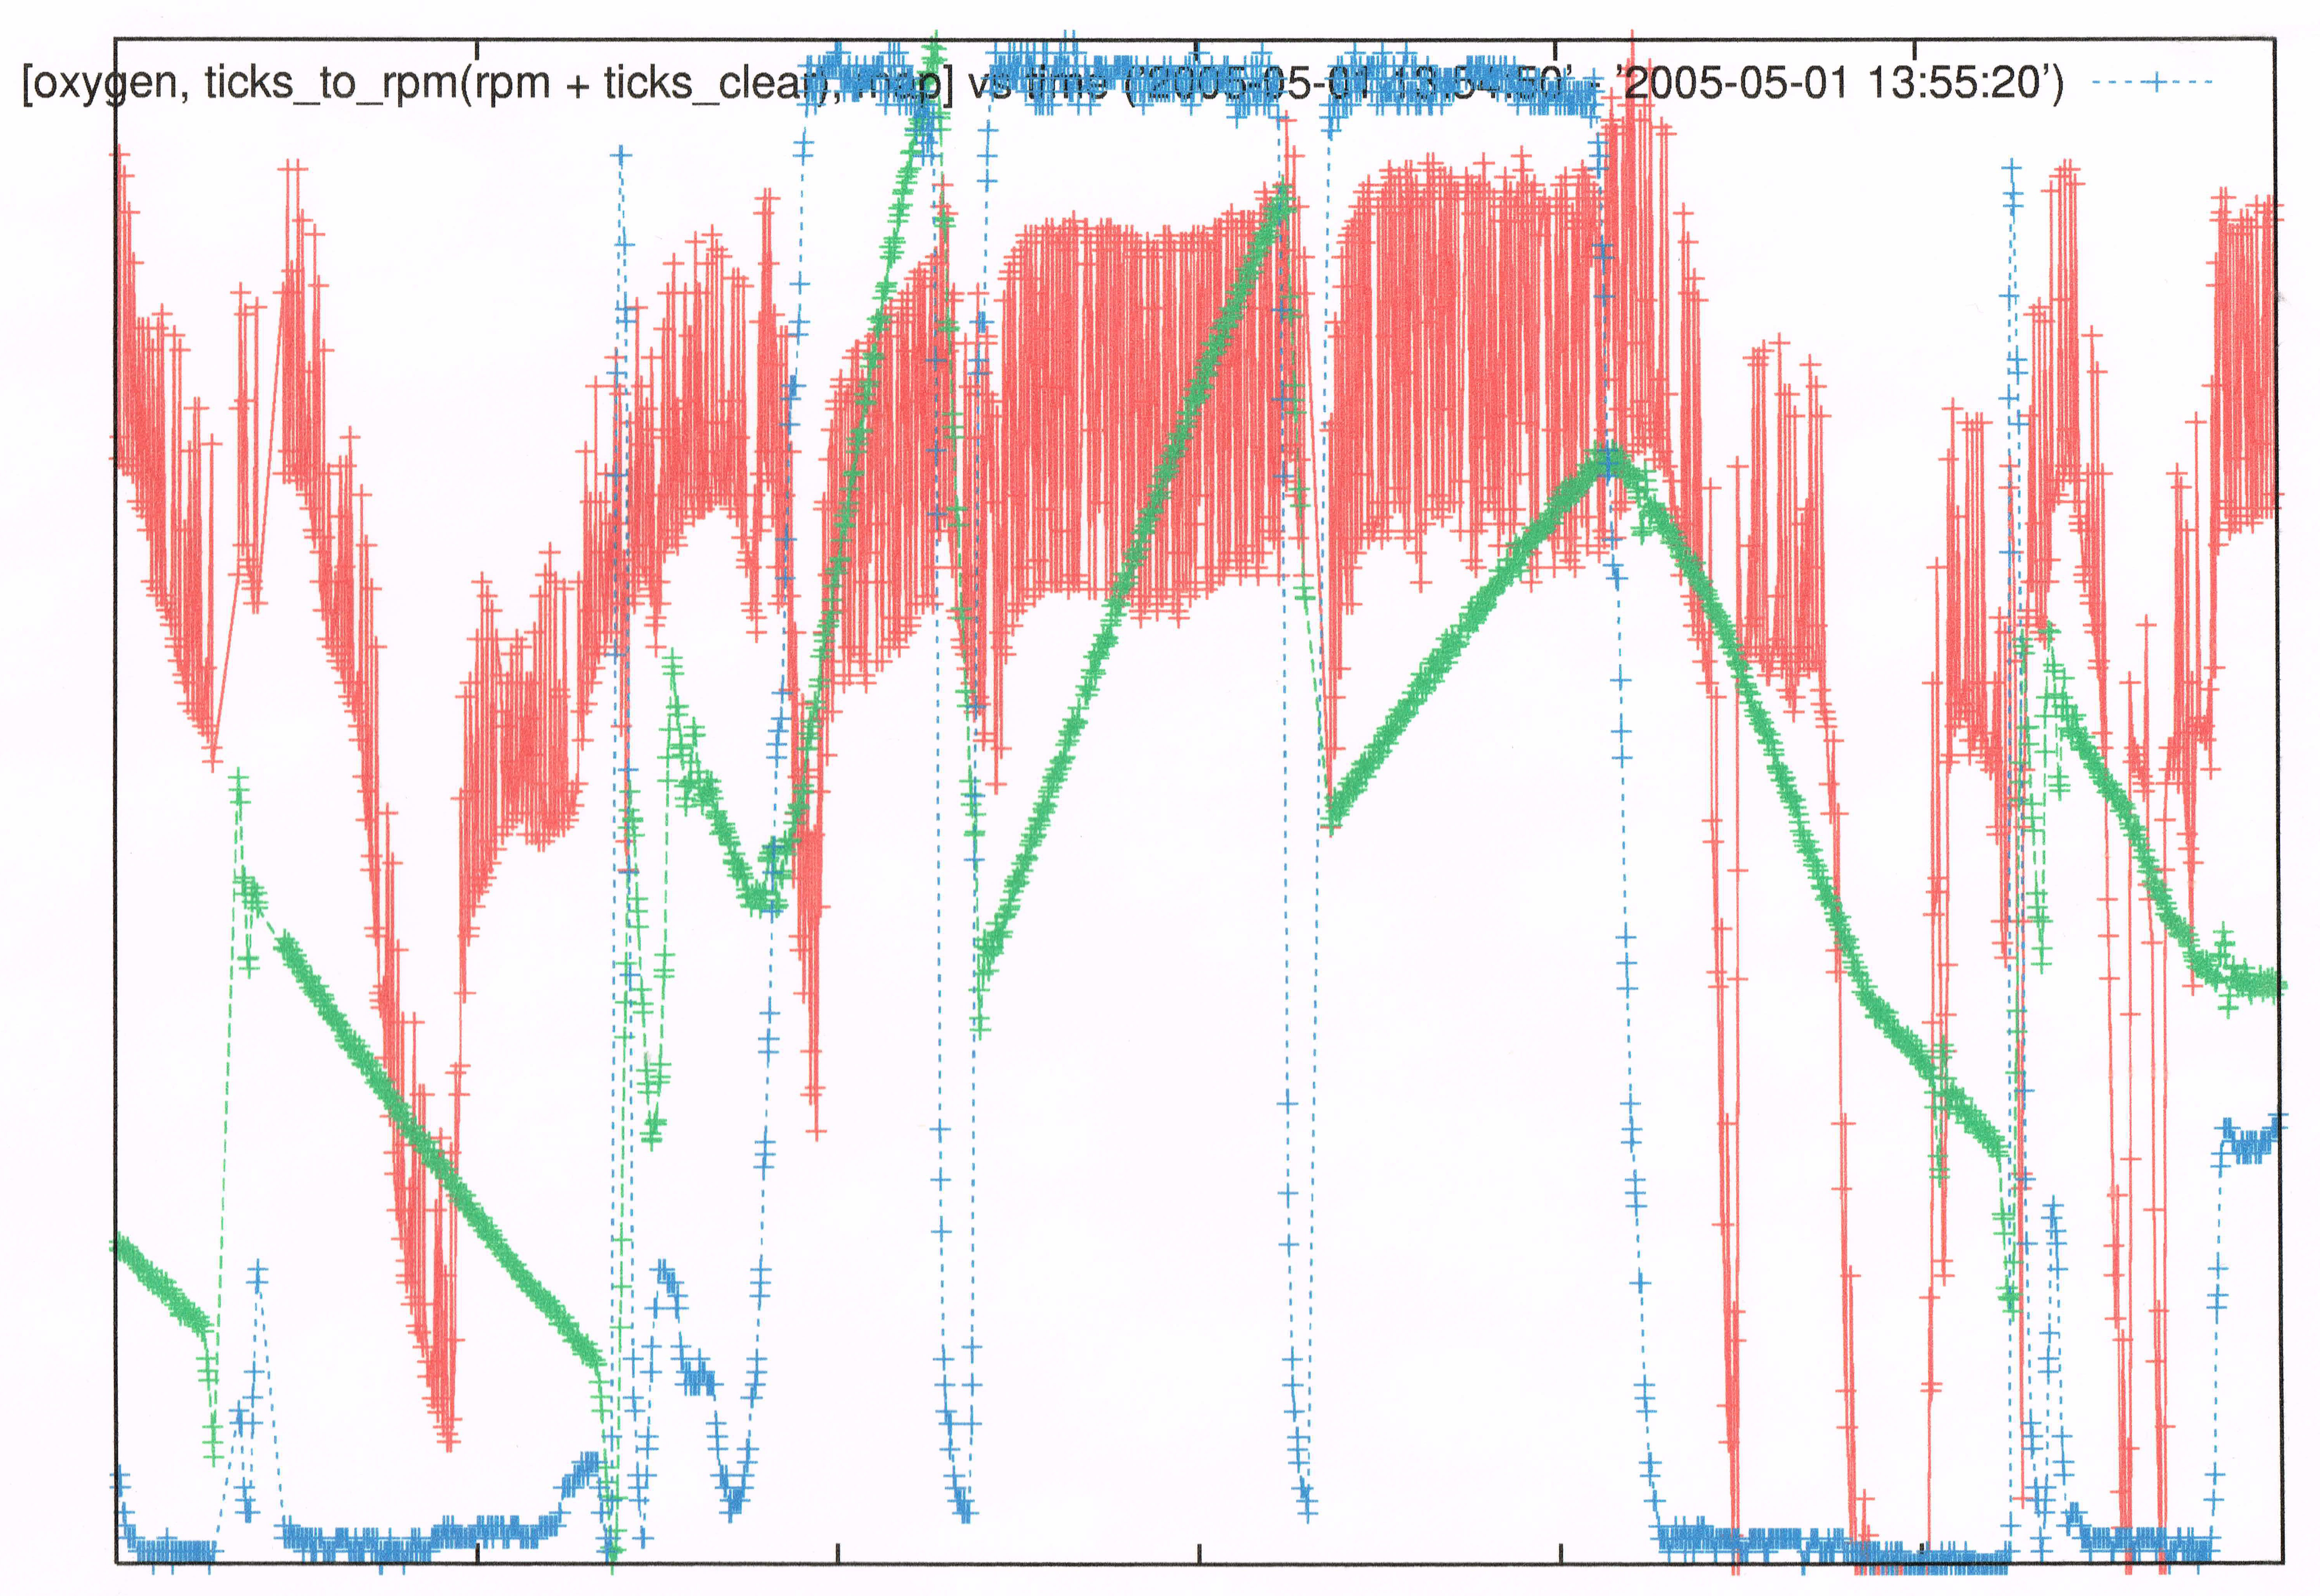
\includegraphics[scale=0.30]{jpg/01111401_mod2}
\begin{itemize}
\item map sensor: blue, O2 sensor: red, rpm: green
\item Full throttle, through three gears.
\item 2005
\end{itemize}
\end{center}
\end{frame}

%\section{McLeod Institute}
\begin{frame}

\frametitle{Current Projects}
\begin{itemize}
\item California State University Chico
	\begin{itemize}
	\item B.S. Electrical Engineering.
	\item Spring 2014.
	\end{itemize}
	% TODO - more detail?
\item McLeod Institute of Simulation Sciences
	\begin{itemize}
	\item CSU Chico research project.
	\item Led by Dr. Crosbie, Dr. Zenor, Dr. Kredo and others.
	\item FPGA based real time simulations.
	\item Grants from The Office of Naval Research.
	\item Electric motor simulations for naval ships and UUV. 
	\item Work with three other students.
	\end{itemize}
\end{itemize}

\end{frame}

%\section{Preview}

\begin{frame}
\frametitle{Preview}
\begin{itemize}
\item Introduction to one of the simulation architectures that were
	developed at McLeod Institute.
\item Problems encountered during its development.
\item Along with solutions.
\end{itemize}
\end{frame}

\section{Simulation Architecture}
\begin{frame}
\frametitle{Background: Simulation Architecture}
\begin{center}
\includegraphics[scale=0.25]{dia/arch1}
\begin{itemize}
\item FPGA
\begin{itemize}
\item Matrix multiplier, core computation engine.
%\item Matrix multiplier used to solve linear models of electric motor.
\item Top level connects the matrix multiplier to the PCIe bus.
\end{itemize}
\item PC
\begin{itemize}
\item Control program can be a test program or user interface such as Simulink.
\end{itemize}
\end{itemize}
\end{center}
\end{frame}

\section{Synthesis Time}

% Convince that development time is long and there is no
% easy way around this problem.
\begin{frame}
\frametitle{Problem: Synthesis Time}
\begin{center}
\includegraphics[scale=0.29]{dia/arch1}
\begin{itemize}
\item Synthesis of HDL code with a 20x20 matrix takes two hours.
\item HDL Simulation?
	\begin{itemize}
	\item Simulation of PCIe bus?
	\end{itemize}
\end{itemize}
\end{center}
\end{frame}

%\begin{frame}
%\frametitle{FIFOs}
%\begin{itemize}
%\item FIFO operation is simple.
%\item For the TX FIFO if it is not full and write is enabled data is written.
%\item For the RX FIFO if it is not empty and read is enabled data is read.
%\end{itemize}
%\end{frame}

\begin{frame}
\frametitle{Solution: FIFO Simulation}
\begin{center}
\begin{itemize}
\item Matrix multiplier and top level change frequently.
\item PCIe bus code rarely changes.
\item Idea: Simulate everything after the FIFO interface.
\end{itemize}
\includegraphics[scale=0.25]{dia/arch1}
\hfill
\includegraphics[scale=0.25]{dia/arch1-fifosim}
\begin{itemize}
\item Frequently changed code can be tested in minutes.
%\item Simple test benches.
\end{itemize}
\end{center}
\end{frame}

\section{FPGA Errors}

\begin{frame}
\frametitle{Problem: Errors Running on FPGA}
\begin{center}
\includegraphics[scale=0.35]{dia/arch1-test_fail}
\end{center}
\begin{itemize}
\item Sporadic errors when running on FPGA.
\item Is the FIFO Simulation not recreating some scenario?
\end{itemize}
\end{frame}

\begin{frame}
\frametitle{Diagnosis: Probe Matrix Multiplication in Hardware}

\begin{itemize}
\item Incorrect results.
\end{itemize}
\[
\begin{bmatrix}
	0.025 & 59.50 & 12.0 & 0.0 \\
	1.5 & 32.7 & 12.0 & 0 \\
	0.025 & 89.50 & 12.0 & 0 \\
	0.0 & 23.001 & 0.001 & 1.01 \\
\end{bmatrix}
\begin{bmatrix}
	0.01 \\
	1.50 \\
	460.0 \\
	60	
\end{bmatrix}
= 
\begin{bmatrix}
1929192 \\
8929282 \\
8273994 \\
1234458
\end{bmatrix}
\]

\begin{itemize}
\item Change test program to use an identity matrix.
\end{itemize}
\[
\begin{bmatrix}
	1 & 0 & 0 & 0 \\
	0 & 1 & 0 & 0 \\
	0 & 0 & 1 & 0 \\
	0 & 0 & 0 & 1 \\
\end{bmatrix}
\begin{bmatrix}
	1 \\
	1 \\
	1 \\
	1
\end{bmatrix}
= 
\begin{bmatrix}
1 \\
1 \\
7378292 \\
9288282
\end{bmatrix}
\]
\begin{itemize}
%\item Matrix coefficients loaded once, could not cause error.
\item Partial transfer of input vector?  Buffer underrun?
\end{itemize}
\end{frame}

\begin{frame}
\frametitle{Update: Include Underrun in FIFO Simulation}
\begin{itemize}
\item First, add underrun condition to FIFO Simulation.
\item Should reproduce error from FPGA.
\item Previously, the FIFO Simulation produced the ideal case.
\end{itemize}
\begin{center}
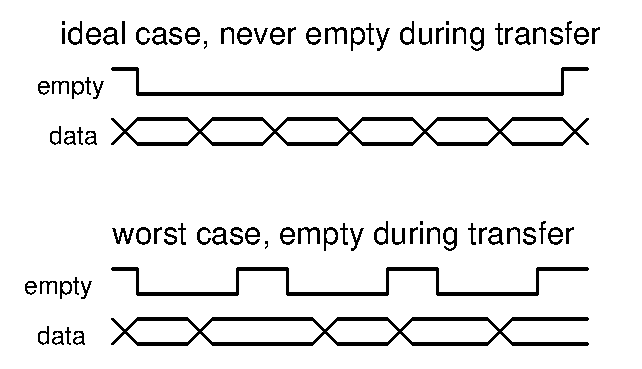
\includegraphics[scale=0.70]{xcircuit/fifosim_timing}
\end{center}
\begin{itemize}
\item Now the FIFO Simulation produces the worst case.
\end{itemize}
\end{frame}

\begin{frame}
\frametitle{Update: FPGA Error Reproduced in FIFO Simulation}
\begin{itemize}
\item Re-run FIFO Simulation tests.
\item Error in FPGA reproduced in FIFO Simulation.
\end{itemize}
\begin{center}
\includegraphics[scale=0.35]{dia/arch1-test_fail2}
\end{center}
\end{frame}

\section{Buffer Underruns}
\begin{frame}
\frametitle{Problem: Buffer Underruns}
\begin{itemize}
\item Why are buffer underruns breaking the top level?
\item Input vector is transferred directly from the FIFO in to the data input.
\item Matrix multiplier reads a new value on each clock edge.
\item \textbf{Operation cannot be paused.}
\end{itemize}
\begin{center}
\includegraphics[scale=0.35]{dia/matrixmult}
\end{center}
\end{frame}

\begin{frame}
\frametitle{Solution: Accumulate Input Vector}
\begin{itemize}
\item Accumulate input vector in top level before transfer to matrix multiplier.
\end{itemize}
\begin{center}
\includegraphics[scale=0.35]{dot/toplevel}
\end{center}
\end{frame}

\begin{frame}
\frametitle{Success: Architecture Operating Correctly}
\begin{center}
\includegraphics[scale=0.35]{dia/arch1-test_success}
\end{center}
\end{frame}

%\section{Electric Motor Simulation}
%
%\begin{frame}
%%\frametitle{Background: Electric Motor Simulation}
%\frametitle{Problem: Incorrect Simulation Results}
%\begin{itemize}
%\item Papers describing electric motor simulation in detail.
%\item Simulations in Matlab.
%\item Reproduce simulation with an FPGA.
%\item Verify the results.
%\end{itemize}
%\end{frame}
%
%%\begin{frame}
%%\frametitle{Problem: Incorrect Simulation Results}
%%\begin{center}
%%\includegraphics[scale=0.35]{dia/arch1-test_success}
%%\end{center}
%%\end{frame}
%
%\begin{frame}
%\frametitle{Solution: Methodically Compare Results}
%\begin{itemize}
%\item Are the model parameters the same?  Motor power rating, number of poles, etc.
%\item Are initial conditions the same? Initial currents and voltages.
%\item Are the generated matrices the same?  $\Phi$ matrix, $\Gamma$ matrix.
%\item Values may not be identical due to different methods.
%\item Tedious process but there is no other way.
%\end{itemize}
%\end{frame}
%
%\begin{frame}
%\frametitle{Success: Simulation in FPGA Agrees}
%\begin{center}
%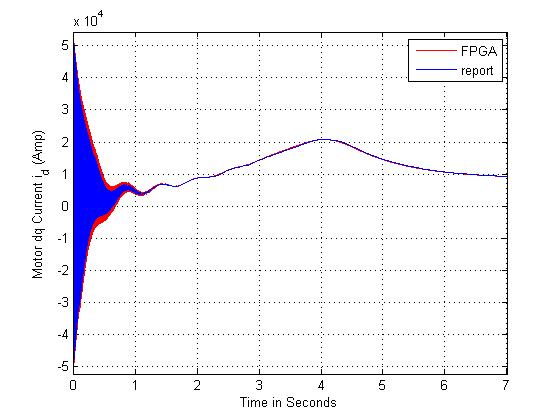
\includegraphics[scale=0.23]{bednar_double_overlay/i_d_double_00001}
%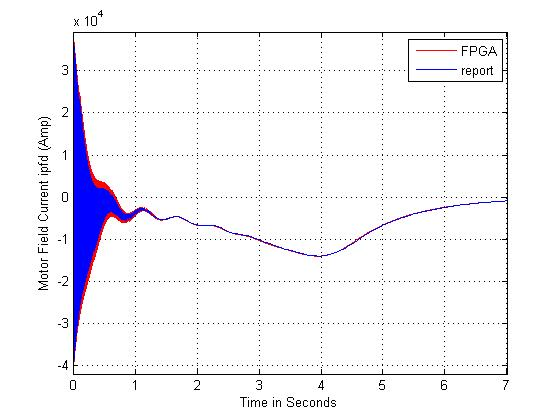
\includegraphics[scale=0.23]{bednar_double_overlay/ipfd_double_00001} \\
%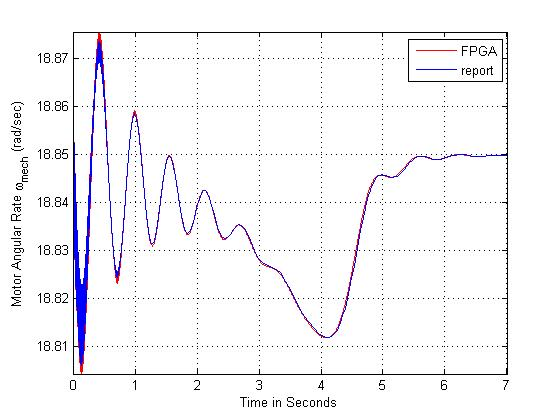
\includegraphics[scale=0.23]{bednar_double_overlay/omega_m_double_00001}
%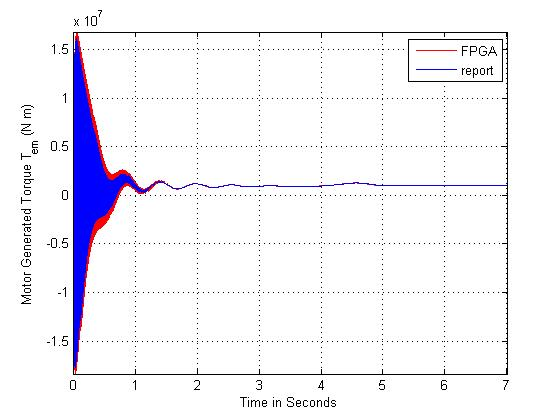
\includegraphics[scale=0.23]{bednar_double_overlay/t_em_double_00001}
%\end{center}
%\end{frame}


% {{{ Questions
\section{Questions}
\begin{frame}[fragile]
\frametitle{}
\begin{center}
\vspace{6em}
Questions? \\
\vspace{5em}
\vspace{2em}
\begin{tabular}{ll}
Jeremiah Mahler \quad\quad\quad & \footnotesize\texttt{<jmmahler@gmail.com>} \\
				& \footnotesize\texttt{github.com/jmahler}
\end{tabular}

\end{center}
\end{frame}
% }}}

\end{document}
